\chapter{Skills}
\label{ch:skills}

Characters use skills to get things done in the game. When the outcome of an action is in doubt, the Gamemaster will ask the player to make a skill test against the relevant skill to see if his character is successful.

\begin{rpg-examplebox}
\begin{description}
	\item[John:] Rurik comes to a large and very deep ravine. Far below he can hear water rushing along the bottom of the ravine, and in front of him are the remains of a rope bridge that has been deliberately broken.
	\item[Rob:] How far across is it?
	\item[John:] About four metres.
	\item[Rob:] Ok, Rurik is going to take a running jump across the ravine.
	\item[John:] Give me an Athletics skill test, since that covers Jumping. You do realise that if Rurik fails he’s facing a very nasty fall?
	\item[Rob:] Yeah, Rurik works that out, but decides to worry about that when and if it happens.  Rurik’s athletics is 60\%.
	\item[] Rob rolls a D100, his red dice (tens) comes up 3 and his white dice (units) comes up 4.
	\item[Rob:] 34, a success. Rurik takes a running jump across the ravine and is now on the other side. What’s there?
\end{description}
\end{rpg-examplebox}

This chapter describes when and how to make skill tests, how to modify skills depending upon the conditions the test is made under, and how to judge tests where two characters are competing against each other. Finally, a list of skills used in the game is detailed.

\begin{figure}[h]
\begin{center}
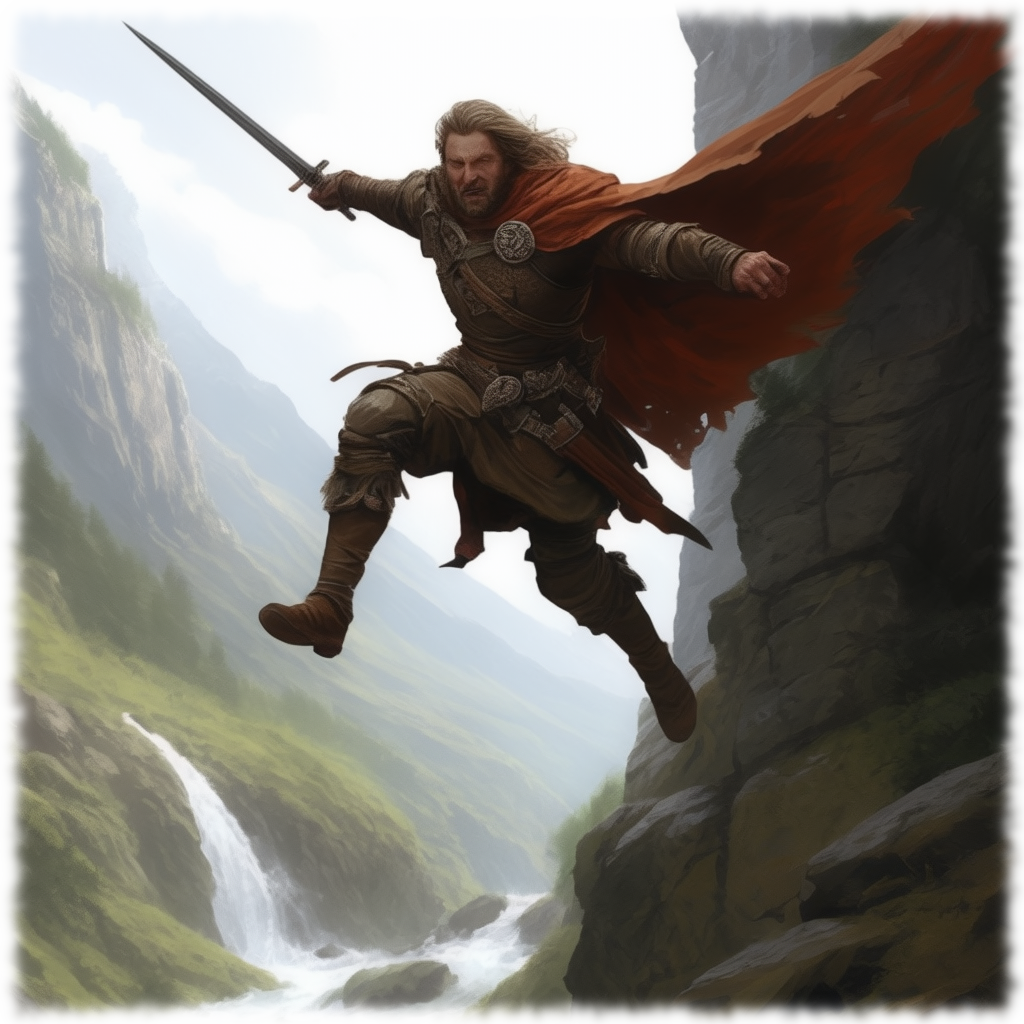
\includegraphics[scale=0.24]{img/ai-images/warrior-jumping.png}
\end{center}
\end{figure}

\section{The Basic Skill Test}
To make a skill test the player first describes what their character is doing. Then they roll a D100 and compare this to the relevant skill’s score. If the dice roll is equal to or less than the skill’s score, the attempt is successful. If the total is greater than the skill’s score, then it has failed. The Gamemaster then describes the result of the character’s success or failure.

Under normal conditions a skill test is asked for when the character is placed on the spot and has to make a successful action under pressure. 

\begin{rpg-examplebox}
An apprentice potter (Craft 25\%) will, day in day out, produce a couple of pots of passable quality if working at his Master’s workshop. Of course, work beyond the skill of the character is still out of their reach, unless the player decides to take the chance with the dice and ask for a skill test.
\end{rpg-examplebox}

If a character has lots of time, has the tools of his trade and is in a sufficiently relaxed environment and state of mind, they complete the task to the best of their ability. 


\begin{figure}[h]
\begin{center}
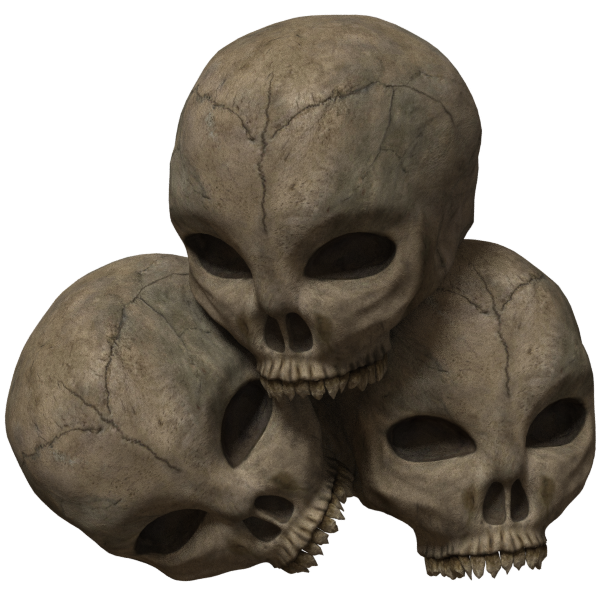
\includegraphics[scale=0.13]{img/SkullPile.png}
\end{center}
\end{figure}

\begin{rpg-examplebox}
A local noble wants an artistic piece of pottery for a grand celebration he is holding later in the month. His servant comes to the potter’s workshop, looking for the Master, who is out. The apprentice sees a chance to gain a good reputation and takes the commission. Knowing that his normal work will definitely not be up to scratch, the player decides to roll the dice in the chance that he can produce something of the standard the noble expects.
\end{rpg-examplebox}

\begin{figure}[h]
\begin{center}
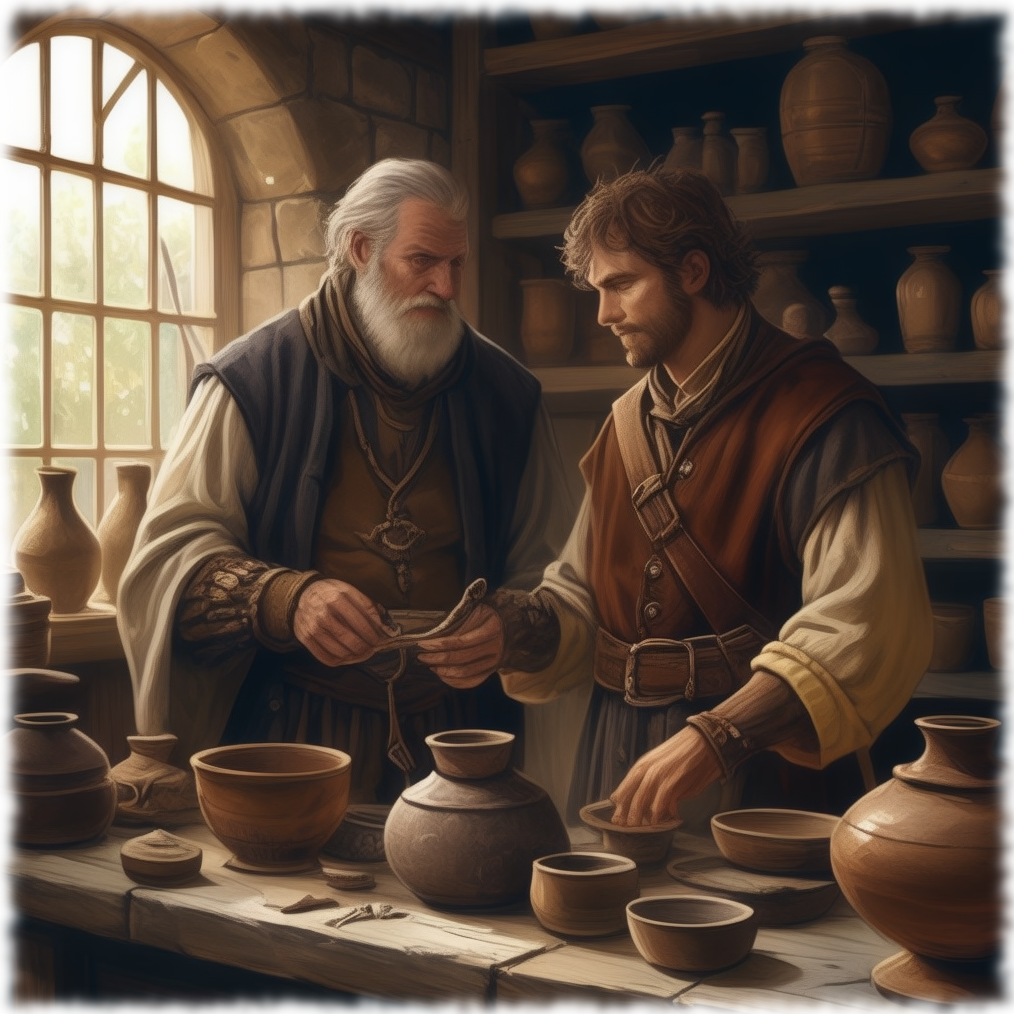
\includegraphics[scale=0.24]{img/ai-images/potter-and-nobleman.png}
\end{center}
\end{figure}


\subsection{Critical Successes}
If the dice roll on a skill test is equal to 01 or is less than 10\% of the modified skill, then a critical success is achieved. 

A critical success has an outcome that far exceeds the expectation of the player when the original skill test was made. It’s the best possible result based upon the player’s original statement of intent.

The actual result of a critical success during a skill test is largely up to the Gamemaster. It normally achieves one of the following results: 

\begin{rpg-list}
\item The task is completed sooner. 
\item The task is completed to a higher degree of expertise than normal. 
\item The task is completed with élan and style, generally impressing witnesses. 
\item The character gains additional information or insight into the task thanks to their brilliance. 
\end{rpg-list}

\begin{rpg-examplebox}
When Rurik is jumping the chasm, his Athletics skill is 60\%  and therefore his chance of getting a critical is 6. Rob rolls a 4, which is less than the 6\% target for a critical success.  As a result, the Gamemaster rules that Rurik easily jumps the chasm with grace that allows him to carry on running without having to pause to catch his breath.
\end{rpg-examplebox}

\subsection{Fumbles}
Whenever a skill test results in a roll of 99 or 00, i.e. the two D10s both come up 0, then the player has fumbled. If the player's modified skill is greater than 100\% then a fumble occurs only with 00.

A fumble is the worst imaginable outcome of the skill test based upon the player’s original description of what their character was planning to do when the skill test was called for.

The actual result of a fumble is largely up to the Gamemaster to decide. It normally results in one of the following mishaps: 

\begin{rpg-list}
\item The task takes twice as long to finish and is still a failure. 
\item The task produces a useless result that actually makes further actions more difficult. 
\item The task fails spectacularly, opening the character up to derision and scorn from witnesses. 
\item The character becomes impeded or even harmed by his failure. 
\end{rpg-list}

Conversely if Rob rolls 00, Rurik not only fails to make the jump over the chasm but goes plunging down the ravine head first. This need not lead to damage and the demise of the character, but they should definitly be at a disadvantage.

There are specific Critical Success and Fumble results for weapon skill tests in combat and Discipline skill tests, which are described in the relevant chapters.


\section{Difficulty}
Modifiers are temporarily applied to the skill for the duration of the test only. A penalty will make the test harder while a bonus makes it easier.  Modifiers are applied before the dice are rolled. For simplicitly they are increments of 20, with $\pm$20 and $\pm$40 being the usual modifiers but more rarely $\pm$60 or even $\pm$80 can be used.

\begin{table}
\begin{center}
\caption{Difficulty Modifiers}
\label{tab:difficulty-modifiers}
\begin{rpg-table}[|l|c|X|]
	\hline
	\textbf{Skill}  & \textbf{Base} & \textbf{Description}\\
	\hline
	Trivial     & +60\%  & The task is trivial under the circumastances and the character should have an almost certain chance of success.\\
	Easy        & +40\%  & The task is much easier than usual and the character should have a high chance of success.\\
	Simple      & +20\%  & The task is simpler than usual and while success is still by no means certain, the character has a boost to their chance of achieving their goal.\\
	Normal      & +0\%   & The skill is unmodified since normal conditions apply.\\
	Difficult   & -20\%  & The character is significantly hindered in their chance of success.\\
	Hard        & -40\%  & The character suffers a serious set back that may make success beyond their reach.\\
	Impossible & -60\%  & The characters is against incredible odds and succeeding is almost impossible.\\
	\hline
\end{rpg-table}
\end{center}
\end{table}

\subsection{Impossible and Automatic Tasks}
Any skill which is modified to 0 or less will automatically fail when tested. Roll dice anyway, since the character can still fumble.

Any skill which is modified to 100\% or greater will automatically succeed when tested. Roll the dice anyway since the character can still critical (10\% of the modified skill) or fumble if the player rolls a 00.

%Masters in a skill (characters with 100\%+ unmodified) never fumble on a skill.


\begin{rpg-examplebox}
Whilst at the Royal Court, Rurik is asked to compose a clever and stimulating poem for the notoriously hard to please Count of Malvon. This is rated as a Hard (-40\%) task. The modifier drops Rurik’s skill of Performance 35\% to -5\%, so Rurik automatically fails the test. However the dice are still rolled because on a roll of 00 Rurik will also fumble his attempt and find himself displeasing the Count.

After displeasing the Count, Rurik tries to hurdle a small wall while being pursued by the Count’s guards. The Gamemaster rules that this is an easy task, +40\%, so Rurik’s Athletics skill of 60\% ends up being increased to 100\%, which gives him a 10\% chance of rolling a critical and impressing the onlooking ladies of the court with his style and grace.
\end{rpg-examplebox}

\subsection{Applying Difficulty Modifiers}
\label{ssec:when-to-apply-difficulty-modifies}
Modifiers should only be applied when they have a significant effect on the character’s chance of success. They should not be doled out for every skill test, since this cheapens their dramatic effect. Only apply a modifier when it is important and brings something to the story. Resist the urge to hand out +10\% here and take {-5\%} there. These little modifiers don’t add much to the player’s chance of success and bring needless fiddly addition and subtraction into play, breaking the player’s immersion in the game.

Broadly speaking, there are three areas where the Gamemaster should modify the player’s skill before a skill test. The three areas are:

\begin{rpg-list}
	\item As a result of the task being inherently easy or difficult.\\
	\item As a result of planning.\\
	\item As a result of good roleplaying.
\end{rpg-list}


\begin{figure}[h]
\begin{center}
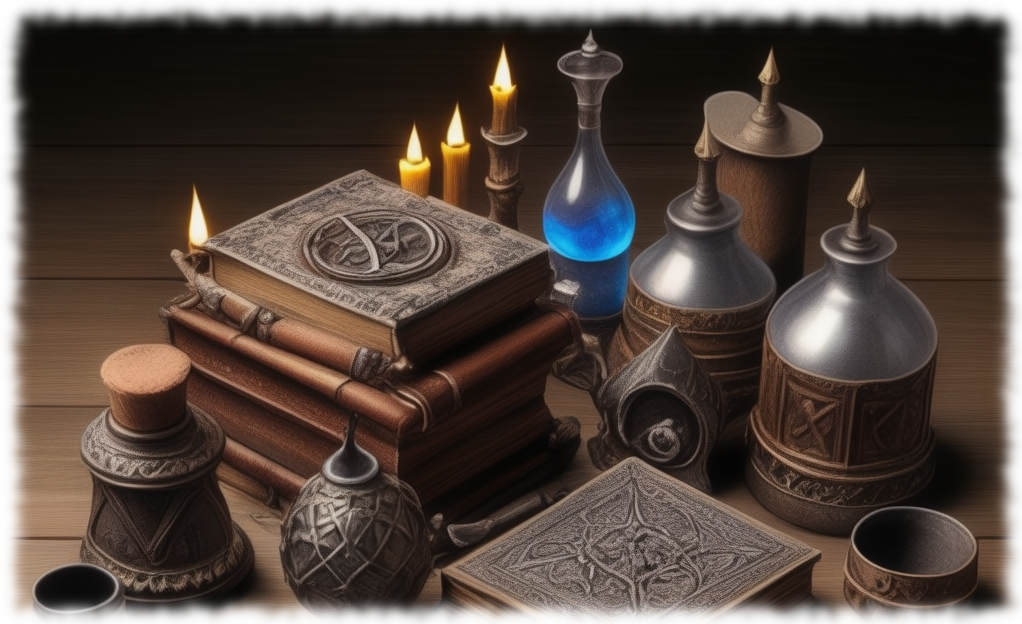
\includegraphics[scale=0.24]{img/ai-images/book-and-bottles.png}
\end{center}
\end{figure}

\subsubsection{As a result of the task being inherently easy or difficult.}
Some things are just naturally easier or harder to do than others. 

For example, climbing a steep cliff with natural hand holds and with the proper equipment (e.g. ropes and iron spikes) is an unmodified task.  Doing the same climb in the pouring rain, makes it Difficult (-20\% to the skill) and if the character has also forgotten his ropes and spikes then this makes it Hard (-40\% to the skill).

In comparison, climbing a cliff where there are numerous ledges, and where the character can rest and actually walk up the cliff in places becomes an Easy (+40\%) skill test.


\subsubsection{As a result of planning}
The Players have outlined how their characters prepares to perform a task well in advance. If their plan is a sound and good one you should make the skill test Easy. Conversely, if the Players have given no thought as to how their characters approach a complex task which really does require preparation and planning, then make the resulting skill test Hard.

\begin{rpg-examplebox}
Several adventuring groups, in search of a lost temple, are about to enter the Badlands, a notoriously harsh wilderness where it is hard to find water and food. The Gamemaster has decided in advance to ask the players to make Natural Lore skill tests, to see how their characters fare in this unforgiving environment.

Flynn’s Riders spend an extra couple of days in the city planning and preparing for the trip. They buy more than adequate supplies and equipment, along with the extra beasts of burden to carry them. Their scholars visit the local Temple of Knowledge and beg, borrow and steal maps of the Badlands, brought back by previous explorers. Finally, they manage to track down a guide, a survivor of a previous expedition, and persuade him to come along.  The Gamemaster awards them a +40\% modifier to their Survival roll.

The Red Hand Gang makes the traditional preparations for any journey. They ensure they have enough supplies, but take no back up mounts or proper traveling clothing. In this case the Gamemaster does not modify their Survival roll on account of their preparation.

Alber’s Lucky Five decide to live up to their name and simply decide, as soon as they hear about the lost temple, to ride out into the Badlands on the horses they arrived on, without replenishing supplies. The Gamemaster modifies their Survival roll by -40\% as a result of their rashness.
\end{rpg-examplebox}



\subsubsection{As a result of Good Roleplaing}
This usually happens for skills that involve some form of communication, like Influence.  When the Player describes the action of their character, the exchange between their character and the non-player character(s) being influenced may be roleplayed out. If the player was entertaining, kept in character and added to the fun of the game, the Gamemaster may award them a +20\%, +40\% or +60\% bonus.  In exceptional circumstances, where the player reduced everyone to tears of laughter, or was outstanding in their portrayal of their character, the Gamemaster may waive the necessity for the skill test completely. Remember good storytelling always comes before any dice rolling. 


\section{Opposed Skill Tests}
Opposed skill tests are made by both characters who are in direct competition with each other. Both characters make the skill tests as normal, rolling 1D100 and attempting to roll equal to or under their skill.

\subsection{One Character Succeeds}
If one character succeeds their skill test and the other fails, then the successful character has won the opposed skill test. 


\subsection{Both Characters Succeed}
If both characters succeed then whoever rolled the highest in their skill test wins the opposed test.  However if one character rolls a critical, while the other rolls an ordinary success, then the character that rolled the critical, which is regarded as a higher level of success, wins. 

\subsection{Both Characters Fail}
Whoever rolled the lowest in their skill test wins the opposed test. In the case of ties for both the Player wins.

\begin{rpg-examplebox}
It’s curfew in the big city and Rurik fancies going to the after hours drinking session at a local tavern. As he heads down the street towards the ale house, he sees a member of the city’s police force, the Watch, walking up the opposite side of the street. Rurik, being Rurik, decides to sneak past the watchman, by creeping up the dark side of the street.

The Gamemaster calls for a Deception skill test from Rurik, since this skill deals with sneaking. Rurik’s Deception skill is only 22\% as he is big, clumsy and trained as a warrior and not a thief. Simultaneously the Gamemaster makes a Perception skill test for the watchman. The watchman’s Perception is 40\%, because this is what he does for a living every night.  Fortunately for Rob, Rurik’s player, the Gamemaster decides that being on the shadowy side of the street significantly helps Rurik, making the test simple (+20\%), which means that Rurik’s Deception is now 42\% for the purpose of this test.

If Rurik rolls a 1 he gets a Critical success and manages to slip past the watchman, regardless of whether he succeeds or not. The watchman would only see Rurik if he rolled a higher Critical himself.

If Rurik rolls a 7 and gets a success and the watchman rolls 55 and fails. Rurik sneaks past him on the darkened side of the street.

If Rurik rolls a 65 and fails and the watchman rolls 30 and gets a success. The watchman spots a shape in the shadows and heads over to investigate.

If Rurik rolls a 15 and succeeds, as does the watchman who rolls a 9, then Rurik wins and evades him because he rolled the highest roll. The watchman thought he saw a shape in the shadows, but it’s gone so quickly that he thinks no more of it.

If Rurik rolls a 65 and the watchman rolls 75, then even though both fail, Rurik wins again because he rolled the lower of the two. Although Rurik stumbled out of the shadows badly at one stage, the watchman is so lost in his own thoughts that he is completely oblivious to Rurik’s blunder. Rurik evades him.
\end{rpg-examplebox}


\begin{figure}[h]
\begin{center}
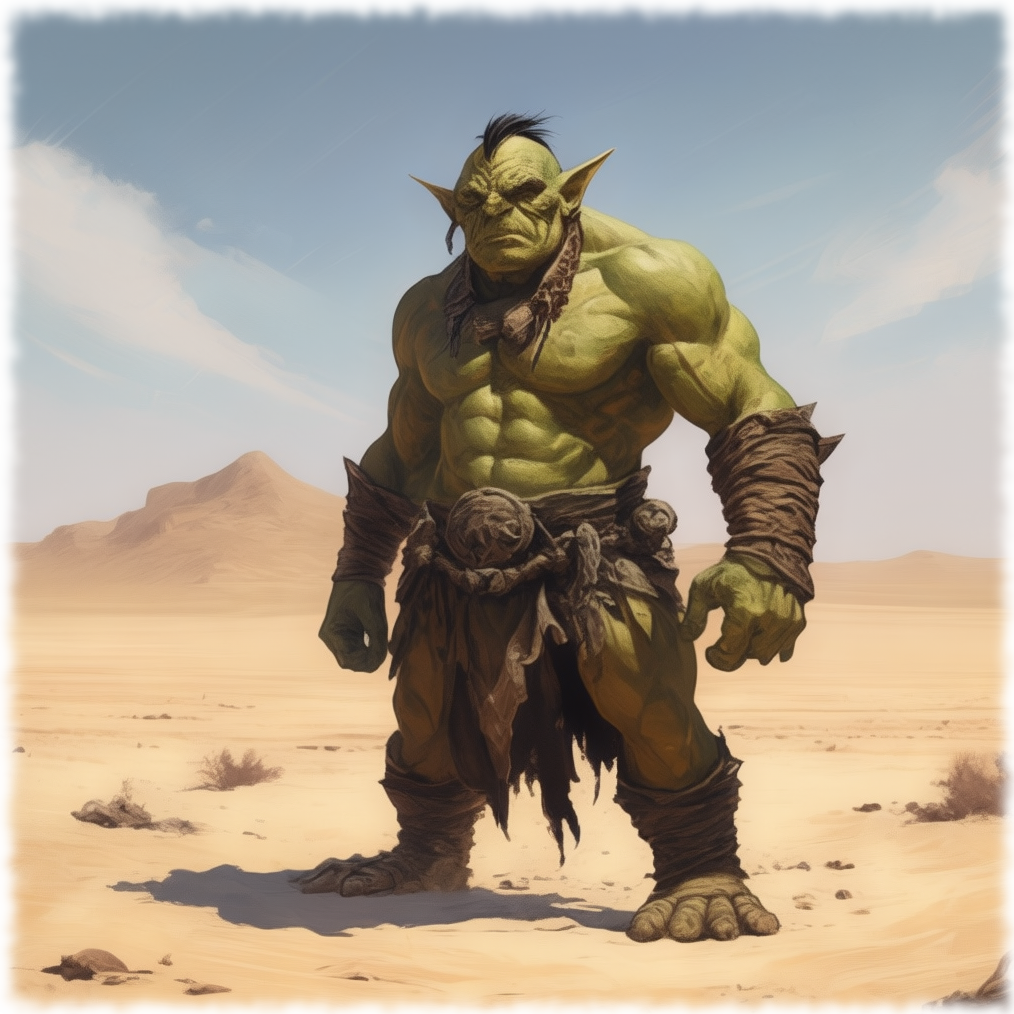
\includegraphics[scale=0.24]{img/ai-images/orc-wrestler.png}
\end{center}
\end{figure}

\section{Very High Skills}
Character’s with Skills over 100\% are considered Masters in their fields and under normal circumstances do not fail and quite often perform tasks that are considered impossible by normal people.

\subsection{Opposed Tests}
In opposed skill tests characters with skills over 100\% are already considered to have succeeded. Therefore to be beaten his opponent needs to score a critical success. Of course the Master may also roll a critical, in which case the highest roll wins.


\begin{rpg-examplebox}
Grazum The Blackheart, an evil Orc Warlord is a Master Wrestler with an Athletics skill of 120\%.  Rurik recklessly challenges him to an arm wrestling contest. Rurik, who has an Athletics skill of 60\%, will automatically lose against Grazum unless Rurik rolls a critical success (6\% or lower).
\end{rpg-examplebox}

\section{Assistance}
Characters will often have the opportunity to help each other during various skill tests. If one or more characters can assist and make a significant contribution then the skill test is one level easier. On rare occasions the assistance will make the skill test two levels easier (GMs discretion).  The assisting character or characters must have the appropriate helping skill at a suitable level determined by the Gamemaster. How high this needs to be is usually dependant on the Difficulty of the test. In most cases as long as the assisting character has a skill of at least Apprentice level (26\%+) then they can help.

\begin{rpg-examplebox}
Rurik is trying to force open an old and mouldy door. If Abnon with an Athletics of 50\% helps him, Rob adds +20\% to Rurik’s Athletics.
\end{rpg-examplebox}


\section{Skill Descriptions}
This is the full list of skills in alphabetical order.

\subsection{Athletics ($DEX+STR$)}
This broad skill covers a range of athletic activities useful to adventuring characters, including acrobatics, climbing, jumping and swimming. 

\begin{description}
	\item[Acrobatics:] This allows a character to perform a variety of gymnastic and balancing tasks, such as tumbling, walking a tightrope or keeping balance on a narrow or unstable ledge. The character can move at half their normal speed across an unstable surface without penalty. To move at a normal rate requires an Acrobatics test. A successful Acrobatics test will also halve the damage suffered from falling. 

	\item[Brute Force:] Brute force is a particular application of Athletics that relies purely on power, with no finesse involved. Brute force basically involves pushing, lifting or dragging. 

	\item[Climbing:] Given enough hand and footholds, a character can climb any surface given enough time without the need for a test. Under normal circumstances, a character can climb or descend one quarter of their Movement per Combat Round (see Chapter 5 Combat for details). A character can double the rate of their climb or descent by making a Hard Athletics test. 

	\item[Jumping:] In general, a successful Athletics test allows a character to jump up to twice their own height horizontally or up to half his own height vertically, as long as he has at least five metres to run first. If they are making a standing jump these distances are halved. For humans, average height is roughly 1.8m which gives a jumping distance of 4m. Penalties for jumping Athletics tests are accrued by trying to jump further. A cumulative –20\% penalty is bestowed for every extra metre the character is trying to jump. If this penalty reduces the skill below 0\% then the character automatically fails, roll to see if they fumble.

	\item[Swimming:] Characters normally swim at half their usual Movement. Athletics tests are only required when conditions are less than ideal – swimming while heavily encumbered or in strong currents for example. 
\end{description}

\subsection{Close Combat ($DEX+STR$)}
This skill deals with the art of hitting things and defending the character with melee weapons, such as swords, clubs, spears, polearms and shields.

\subsection{Craft ($INT+10$)}
The Craft skill is actually several separate skills (such as armourer, baker, basket weaver, blacksmith, bowyer, brewer, butcher etc) grouped under a single heading which must be improved separately. It measures the character’s ability to make and repair items.
As a very rough guide it takes one day per 50 SP to produce an item. The base cost of the item, in materials needed, is 50\% of the listed finished cost.

\subsection{Culture ($INT+10/INT$)}
Each Culture skill is used to provide information about the common world view of that group of people (or creatures). This includes history, politics, weather cycles, geography, superstitions and popular mythology. 

Culture (Own) is the world view of the people that the character is born into, which is why the character gets a +10. All other foreign or alien cultures are Culture (Other).

\subsection{Deception ($DEX +INT$)}
Deception covers the arts of:
\begin{description}
	\item[Disguise:] used to change a character’s appearance and adopt a different outward persona. 
	\item[Sleight:] used to hide or take objects, without drawing undue attention. 
	\item[Stealth:] used whenever a character attempts to personally evade detection by another character. This usually happens when a character either tries to move quietly past an enemy, hide from one, or performs a combination of both.
\end{description}

These tests are opposed by the Perception skill and are modified according to the situation. 

\subsection{Dodge ($DEX+10$)}
The Dodge skill is used to avoid incoming objects that are swung or thrown at the character. The Dodge skill is normally used when a character attempts to dodge an incoming blow in combat or a physical hazard that can be avoided, such as falling masonry. 

\subsection{Driving ($DEX+INT$)}
If a character is driving a wagon, chariot or similar vehicle at not more than walking pace across flat terrain, a Driving skill test will never be required. Skill tests are required when a character wants to do something out of the ordinary with a vehicle, such as traverse treacherous terrain, jump obstacles and so on.

\subsection{Engineering ($INT+10$)}
This skill is used to design, build, activate, repair, sabotage or disassemble large mechanisms or constructs such as siege machines, city gates and drawbridges, mine-shafts, sailing ships and so forth. 

\begin{figure}[h]
\begin{center}
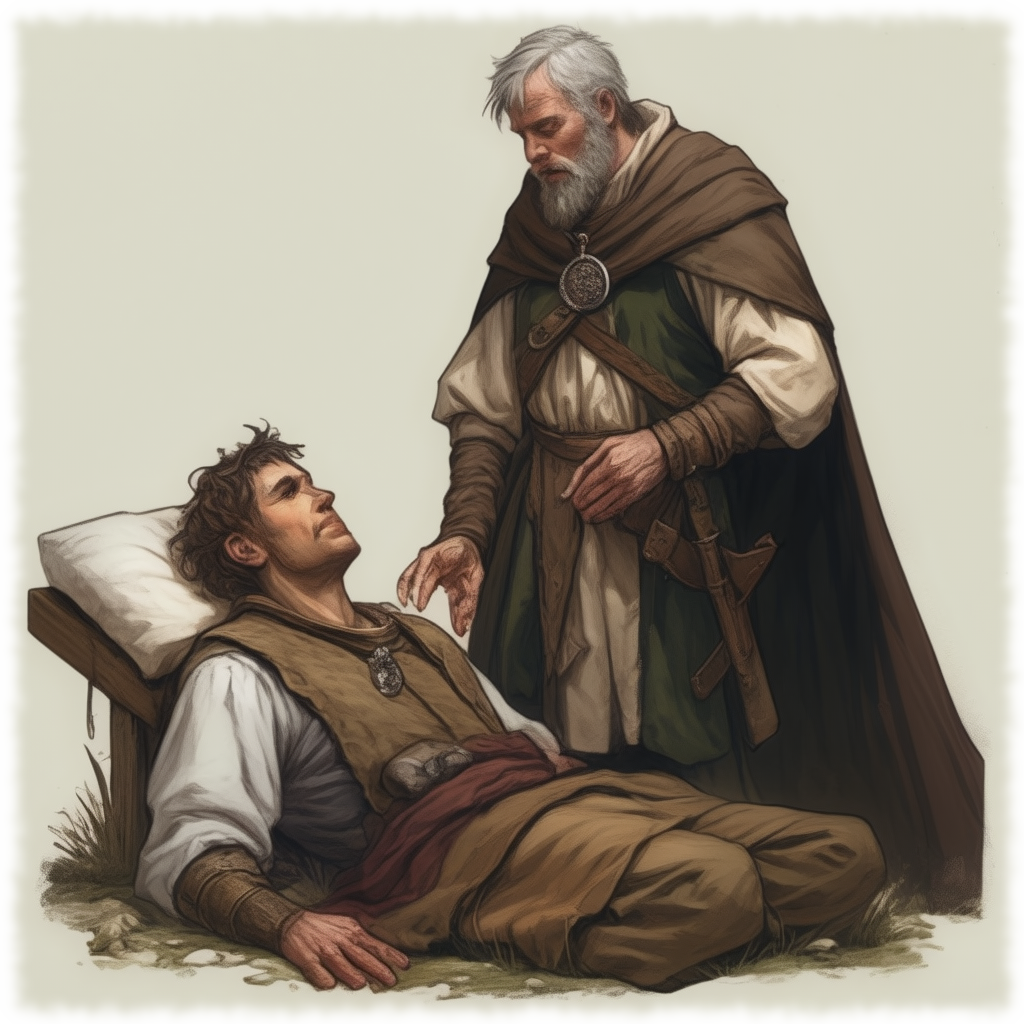
\includegraphics[scale=0.24]{img/ai-images/healer-tending.png}
\end{center}
\end{figure}

\subsection{Healing ($INT+10$)}
Use of this skill without a healer’s kit incurs a -40\% penalty. Each use of the Healing skill generally takes a few minutes to perform. Both characters must remain stationary and may not use Combat Actions or Reactions while this occurs or they will lose the benefits of the healing. Typical types of injuries or ailments that may be treated are listed below:

\begin{description}
\item[Unconsciousness] A successful Healing test can revive a character from unconsciousness, though drugged patients may inflict a penalty on the Healing test.
\item[Minor Injury] A successful Healing test on a Minor Injury will heal 1D4 Hit Points. 
\item[Stabilise Major Wound] A successful Healing test on a Major Wound will not restore the lost Hit Points. This Healing merely stabilises the patient enough so that they will not die of blood loss.
\item[Curing Diseases] A successful Healing test allows a diseased patient to add a bonus to his next opposed test of Resilience versus disease Potency to resist the disease. The bonus is equal to the healer’s Healing skill divided by 10 (the critical success range).
\item[Curing Poisons] A successful Healing test allows a poisoned patient to attempt a second opposed test of Resilience versus poison Potency. The patient gains a bonus to their Resilience skill equal to the healer’s Healing skill divided by 10 (the critical success range).
\item[Surgery] Other than magical healing, successful Surgery is the only way that a character can recover from a Major Wound. Once a successful Healing test has been made to quench the bleeding of a Major Wound, a successful Healing test can attempt to set broken bones, stitch together rent flesh and restore the wound location so that it is on the road to recovery. As long as the Healing test is a success, the stricken character gains one hit point and will begin to heal as normal.
\end{description}

The use of Healing requires suitable medical equipment such as bandages or salves or appropriate improvised alternatives. 


\subsection{Influence ($CHA+10$)}
This is the art of verbally persuading another character to do what you want. Characters can use both logical and/or emotional arguments.  If successful in an opposed skill test, the character’s audience is temporarily swayed in favour of the character’s argument. In time they may understand that they were fast talked, bamboozled or hoodwinked and their judgement clouded, but in the short term they go along with what the character suggests.  Influence can never be used to get a character to act against their instinct for self-preservation.

Influence skill tests are normally opposed by a Perception, Persistence or Influence skill. They are further modified by how much a character is trying to change an opponent’s mind. Influence skill tests are often modified by how well the player roleplays the exchange (see When to Apply Difficulty Modifiers in page~\pageref{ssec:when-to-apply-difficulty-modifies}).

Influence tests are either applied to individuals, where each character rolls individually against the Influencer, or against crowds, were one roll is made to resist based upon an average Persistence for the entire crowd.


\subsection{Language ($INT+50/INT$)}
The Language skill is a separate skill for each language the character knows. Their native language gets a +50\%.

Every character with a Language skill of 50\% or more is fluent in that language, although they are likely to have an accent if it is not their native language. 

A score in a Language skill of 80\% or more will mean the character can also read and write in that language.


\subsection{Lore ($INT$)}
The Lore skill is actually an umbrella term for several different skills, each of which must be improved separately. 

Each Lore skill defines an area of knowledge for the character and skill tests are made whenever a player wants to see if their character knows something about the subject at hand. 

Possible Lores is only limited by a player’s imagination. A list of potential study areas of Lore is listed here:  alchemy, art, astronomy, gambling, geography, heraldry, law, logistics, military tactics, philosophy, poisons.

\begin{figure}[h]
\begin{center}
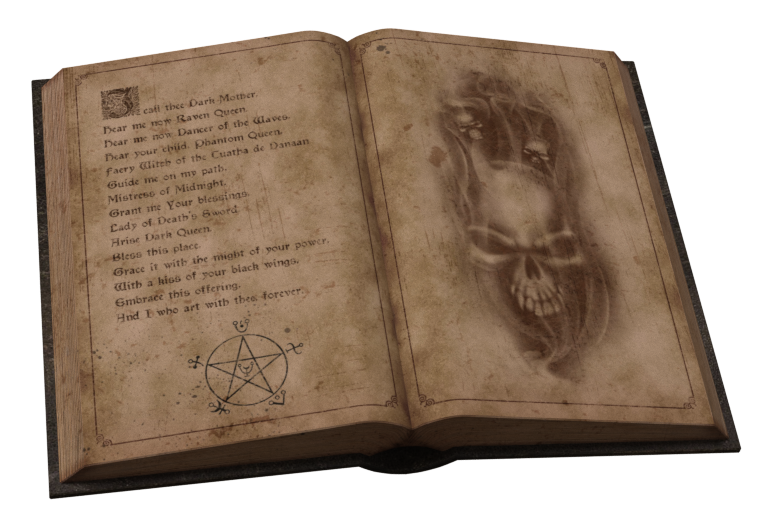
\includegraphics[scale=0.2]{img/OpenBook.png}
\end{center}
\end{figure}


\subsection{Mechanisms ($DEX+INT$)}
Usually, a character will simply make a Mechanisms test in order to succeed at assembling or disassembling a device, with appropriate bonuses or penalties decided upon by the Gamemaster. If a device has been designed to specifically resist attempts at disassembly, the Mechanisms test becomes opposed by the Mechanisms skill of the character that created it. 

Mechanisms is also used for picking a lock or disassembling a trap. This usually takes at least one minute (12 Combat Rounds) to perform, whereas larger or particularly complex devices will take longer.

\subsection{Natural Lore ($INT+10$)}
Broadly speaking this Lore deals with the character’s knowledge of the natural world. It covers several specialist areas.
\begin{description}
	\item[Animal:] This covers the ability to recognise an animal, know its feeding habits, breeding cycle, habitats and so on. A character with a skill of at least 50\% may try to domesticate a wild animal, making a skill test after every full week of training. If the character also has a Riding skill of at least 50\% and the animal is capable of being ridden, they may train the animal to ride during this period. The character may later train the animal not to panic in battle and to strike at his enemies. This takes a further period of training, with the character making a skill test at the end of each week to succeed. 
	\item[Plant:] A character can identify plants in the wild, discover good places to grow crops, decide which plants are edible and what unusual properties they may possess.
	\item[Mineral:]  This skill allows the character to detect precious metals and stones, detect fault lines and other dangerous features in the rock.
	\item[Survival:] One Survival test will be required every day that a character lacks either food, water or a safe place to sleep. Success indicates the character manages to find whatever they are lacking – failure means they will go without which, over several days, could result in very serious consequences. Survival tests are not used when the character is in a city or town. 
	\item[Tracking] A character can track in the wilderness and is able to locate the tracks of a specific creature and follow them. A test must be made to locate the trail and then again every ten minutes they are being followed. 
	\item[Weather:] The character can predict basic changes in the weather.
\end{description}

\subsection{Perception ($INT+POW$)}
The Perception skill is used to represent the five senses of the character when detecting objects or other characters. For example, a common use of the Perception skill is as a straight skill test to detect hidden objects in a room, or as an opposed test to detect a hidden character.

\begin{figure}[h]
\begin{center}
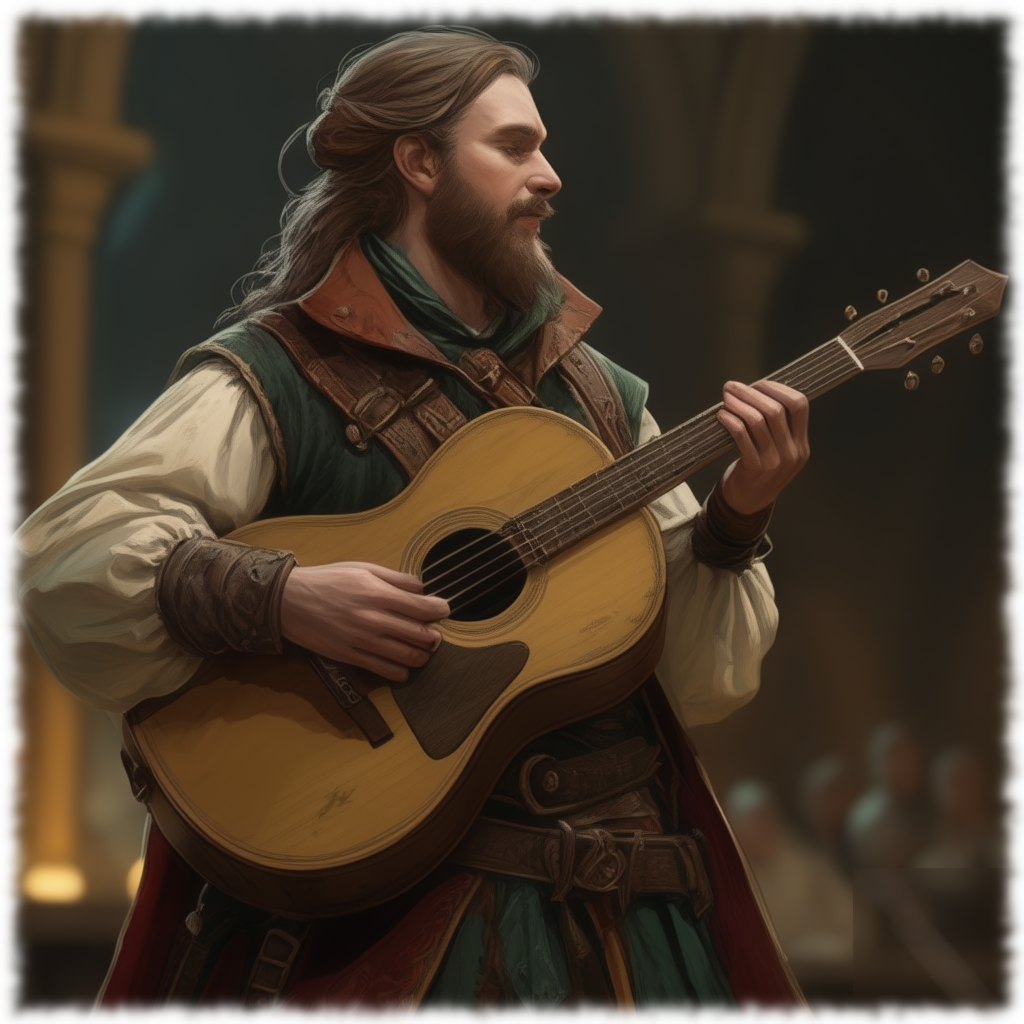
\includegraphics[scale=0.24]{img/ai-images/bard.png}
\end{center}
\end{figure}

\subsection{Performance ($CHA+10$)}
A successful test with this skill will result in the audience or partner being pleased by the character’s performance.  This skill covers acting, composing poetry, dancing, singing, readings and playing an instrument. 

\subsection{Persistence ($POW+10$)}
Persistence represents a character’s mental willpower. It is used to resist the effects of magic and often against another character’s attempt to use the Influence skill against them.  

\subsection{Ranged Combat ($DEX+INT$)}
This skill covers the use of missile weapons, such as bows, crossbows, thrown spears and thrown daggers. It is covered in more detail in the Combat chapter.

\subsection{Resilience ($CON+POW$)}
This is a measure of how physically tough a character is. The higher a character’s Resilience, the more likely they are to handle adverse physical conditions, such as weathering a vicious sandstorm, surviving in a drought, or overcoming the effects of poison or disease. 


\subsection{Riding ($DEX+POW$)}
If a character is riding a creature with the help of saddle and stirrups, at not more than a walking pace across flat terrain, then a Riding test will never be required. Tests are required when a character wants to do something out of the ordinary with a mount – such as traverse treacherous terrain, jump obstacles, ride bareback and so on. 

%Riding can also be used to drive wagons and chariots, etc.


\subsection{Sailing ($DEX+INT$)}
This covers small water-borne craft propelled manually by oars or paddles, commonly known as boats, and larger craft  powered by sail or rows of oars. Travelling across calm water does not usually require a skill test but adverse conditions such as currents and weather can bestow penalties. 

\subsection{Streetwise ($CHA+POW$)}
Streetwise allows a character to find fences for stolen goods, black markets and general information. Such uses of Streetwise normally require a minimum of 1D4 hours.  Streetwise also covers following people down crowded city streets without them being noticed.

\subsection{Trade ($INT+10$)}
\label{ssec:trade}
This skill is primarily used when characters trade, barter or otherwise negotiate over the sale of goods. In such transactions a successful Opposed Test using the Trade of the buyer versus the Trade of the seller is needed for the buyer to get the best deal.  If the buyer wins they get a discount; -10\% for a success, -20\% for a critical. If the seller wins they can sell the item for more; +10\% for a success and +20\% for a critical. If the opponent fumbles their roll, double the increase or decrease.

The Trade skill also enables the character to determine the value placed on something by others; estimating its market value. Particularly common or obscure objects might give a bonus or penalty to the skill test. Success will allow a character to guess the average monetary value of the object, normally guessing accurately to within 10\% of its actual value.  


\subsection{Unarmed Combat ($DEX+STR$)}
This skill covers the use of natural attacks. For humans this is punching and kicking (1D3 damage) as well as grappling. Non-human characters may also have bite, horns, claw and tail attacks. 


